\section{Background}
\subsection{}

\begin{frame}
\frametitle{Project Background}

Ongoing research at the Center for Tropical Research (CTR) at UCLA seeks to identify patterns of continental scale migratory connections 

\begin{itemize}
\item Current methods are too coarse for most applications
\item Large amounts of data are available ( \textgreater{}150,000 feather samples from \textgreater{}500 species)
\item Proposed approach uses genetic and isotopic markers to achieve much greater accuracy
\end{itemize}

\end{frame}


\begin{frame}
\begin{center}
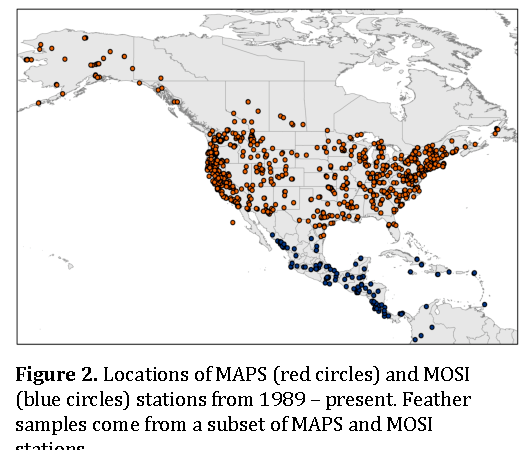
\includegraphics[width=3.5in]{scat/pics/background/sampling_locs.pdf}
\end{center}
\end{frame}



\begin{frame}[shrink]
\frametitle{Species of interest}

\begin{columns}[c]
\column{0.33\textwidth} Hermit Thrush\\
\column{0.33\textwidth} Swainson's Thrush\\
\column{0.33\textwidth} Wilson's Warbler\\
\end{columns}

\vspace{5mm}

\begin{columns}
\column{0.33\textwidth}
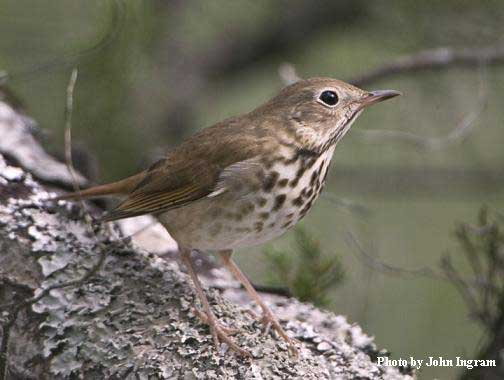
\includegraphics[width=1.25in]{scat/pics/background/hermit_thrush.jpeg}
\column{0.33\textwidth}
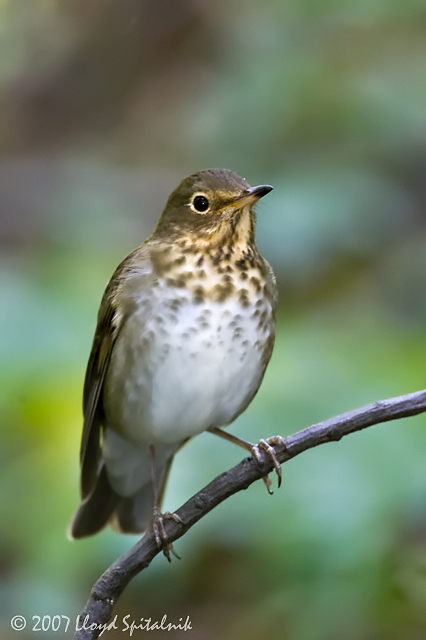
\includegraphics[width=1in]{scat/pics/background/swainsons_thrush.jpeg}
\column{0.33\textwidth}
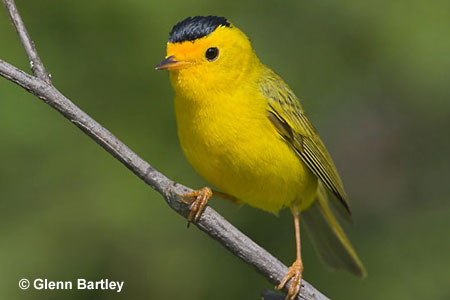
\includegraphics[width=1.25in]{scat/pics/background/wilsons_warbler.jpeg}
\end{columns}

\vspace{5mm}

\footnotesize{
\begin{columns}
\column{0.33\textwidth}
138 Individuals\\
14 Locations\\
6 Loci\\
9-27 Alleles
\column{0.33\textwidth}
162 Individuals\\
7 Locations\\
5 Loci\\
9-23 Alleles
\column{0.33\textwidth}
163 Individuals\\
8 Locations\\
9 Loci\\
15-31 Alleles
\end{columns}
}
\end{frame}



\begin{frame}
\frametitle{Previous work}

\footnotesize{
Wasser, et. al [2004] developed an approach for assigning genetic samples from illegal ivory shipments to geographic locations based on a model of microsatellite allele frequencies in elephant populations throughout africa.
}
\begin{center}
\includegraphics[width=2.5in]{scat/pics/background/wasser.pdf}
\end{center}

\end{frame}

\begin{frame}
\frametitle{SCAT - Smoothed and continuous assignment test }
\begin{itemize}
\item Originally developed by Matthew Stephens, C++ command line tool
\item Built an R package, Rscat, based on this code using Rcpp
\begin{itemize}
\item Core MCMC functionality rewritten using Armadillo
\item Added functionality for visualization and diagnostics
\item Improvements in the underlying model
\end{itemize}
\end{itemize}

\vspace{5mm}

\begin{columns}
\column{0.5in}
\column{0.5in}

\includegraphics[width=0.4in]{scat/pics/background/R_logo.jpeg}
\column{2.25in}

\includegraphics[width=2.25in]{scat/pics/background/armadillo.jpg}
\end{columns}

\end{frame}